\documentclass[tikz,border=6pt]{standalone}
\usepackage{pgfplots}
\pgfplotsset{compat=1.18}

\begin{document}
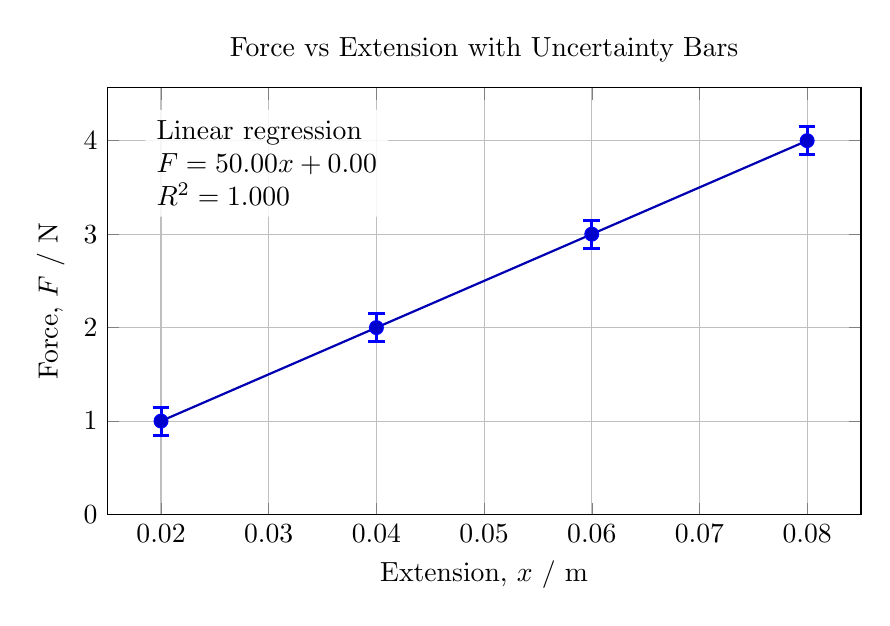
\begin{tikzpicture}
\begin{axis}[
  width=0.92\textwidth,
  height=7cm,
  title={Force vs Extension with Uncertainty Bars},
  xlabel={Extension, $x$ / m},
  ylabel={Force, $F$ / N},
  grid=both,
  ymin=0,
  xmin=0.015,
  xmax=0.085,
  scaled x ticks=false,
  scaled y ticks=false,
  xticklabel style={/pgf/number format/fixed,/pgf/number format/precision=3},
  yticklabel style={/pgf/number format/fixed,/pgf/number format/precision=1},
]
\addplot+[
  only marks,
  mark=*,
  mark size=2.5pt,
  error bars/.cd,
    y dir=both,
    y explicit,
    error bar style={line width=1.1pt},
    error mark options={rotate=90,mark size=3pt,line width=1.1pt},
]
coordinates {
  (0.020,1.00) +- (0,0.15)
  (0.040,2.00) +- (0,0.15)
  (0.060,3.00) +- (0,0.15)
  (0.080,4.00) +- (0,0.15)
};
\addplot[
  domain=0.020:0.080,
  samples=2,
  thick,
  color=blue!70!black,
] {50*x};
\node[
  anchor=north west,
  fill=white,
  fill opacity=0.85,
  text opacity=1,
  rounded corners=2pt,
  inner sep=4pt
] at (rel axis cs:0.05,0.95) {\shortstack[l]{Linear regression\\$F = 50.00x + 0.00$\\$R^2 = 1.000$}};
\end{axis}
\end{tikzpicture}
\end{document}
